\section{Fast Compression}\label{sec:fast-compression}

\textbf{Page budget: 3 pages?}

\begin{outline}

  Background (about 1 column)
  \begin{itemize}
  \item Voxelization \status{[Done]}
  \item Octree basics: also describe Octree coding \status{[Done]}
  \item RAHT algorithm \status{[Done]}
  \item Entropy coding \status{[Done]}
  \end{itemize}

  \eduardo{there are various resolution levels 3DGS encoder: voxelization, geometry octree coding, attribute transforms, attribute RLGR. 3DGS decoder: attribute inverse RLGR, geometry octree decoding, attribute inverse RAHT. For this 3DGS encoder and decoder, there are dependencies (e.g., need to do voxelization first), for decoder need to decode geometry first before inverse raht, but octree decoding can be parallel with RLGR decoding. Then there is the second level of parallelization, which is  parallel RAHT/inverseRAHT, prelude, RLGR, octree coding/decoding.}

  Octree coding: (sub-section, about 2 pages) \status{[Done]}
  \begin{itemize}
  \item Describe standard octree encoding algorithm (tree construction, bitstream generation) (sequential version); make the point here that this needs a voxelized representation (we do this in the GPU) \status{[Done]}
  \item Show a table of quote/approaches from related work about how difficult it is parallelize this. \status{[Done]}
  \item Before explaining our idea: describe morton code \status{[Done]}
  \item Key idea: morton code enables $O(1)$ parent-child determination (show using a figure) \status{[Done]}
  \item How to parallelize Octree encoding: \status{[Done]}
    \begin{itemize}
    \item Tree construction: show by example; \status{[Done]}
    \item Bitstream construction: show by example \status{[Done]}
    \end{itemize}
  \item Detailed algorithm with listing and discussion of the algorithm \status{[Done]}
    \begin{itemize}
    \item But when you describe this, organize it in a template so that for subsequent algorithms, all that needs to change is the code/steps executed at each node/at each level of the parallelism \status{[Done]}
    \end{itemize}
  \end{itemize}

  RAHT prelude and encoding (about a page) \status{[Done]}
  \begin{itemize}
    \item Show a simple example for what the prelude and encoding do
    \item Describe the detailed algorithms using the template discussed above.
      \begin{itemize}
      \item Describe inputs and outputs
      \end{itemize}
  \end{itemize}

  Quantization (half a column) \status{[Done]}
  \begin{itemize}
  \item Background: on what quantization is and how it relates to quality
  \item Briefly describe how we do quantization
  \end{itemize}

  Entropy coding (half a column) \status{[Done]}
  \begin{itemize}
  \item Describe inputs and outputs
  \item Describe how we do RLGR parallelism: block-based to leverage GPU cores
  \end{itemize}

  Decoding: \status{[Done]}
  \begin{itemize}
  \item Explain that this is the reverse
  \item Describe what metadata the encoder needs to send
  \end{itemize}
      
\end{outline}


In this section, we describe each component of the \gsnfs compression pipeline and how we parallelize them. We first provide an overview of the algorithms in that we are take inspiration from G-PCC.

\subsection{Background}\label{sec:background}
\parab{Voxelization.}
A voxel is a volumetric pixel in 3D that represents a discrete cube, a unit on the regular grid in 3D space.
%
In the process of voxelization, the points are partitioned into voxels, and the attributes associated with the 3D points in a voxel are aggregated.
%
Voxelization is often used as a preprocessing step for 3D compression algorithms, as it provides a structured format that can be efficiently encoded.
%
Now, consider a set of $N$ Gaussians for a \gs model with 3D position $V = [v_i \in \mathbb{R}^3]_{i=1}^N$ and other attributes given $A = [a_i \in \mathbb{R}^C]_{i=1}^N$, where $C$ is total dimension across opacity, scales, rotation, and color.
%
First, we voxelize the 3D space into a regular grid of dimension $2^J \times 2^J \times 2^J$ and map each Gaussian to an integer voxel of unit cube size where the voxel center has coordinate $\hat{v}_i \in \{0, \dots, 2^J-1\}^3$; $0$ and $2^J-1$ represents the minimum and maximum coordinate of a tight bounding box of the \gs model, respectively.
%
Since multiple Gaussians can fall into the same voxel, we merge them by averaging their attributes.
%
Both voxelization and merging can be parallelized on GPU by launching one thread per Gaussian, which computes the voxel coordinate and atomically accumulates the attributes into the corresponding voxel.
%
This process reduces the number of Gaussians and improves compressibility. The voxelized \gs model has $\hat{N}_v$ unique gaussians, where position of each gaussian lies exclusively at the center of a voxel with its averaged attribute.

\eduardo{also say that voxelization enables the subsequent compression steps. If data was not vowelized, RAHT does not exist.}

\parab{Octree coding.}
\begin{figure}[t]
  \centering
  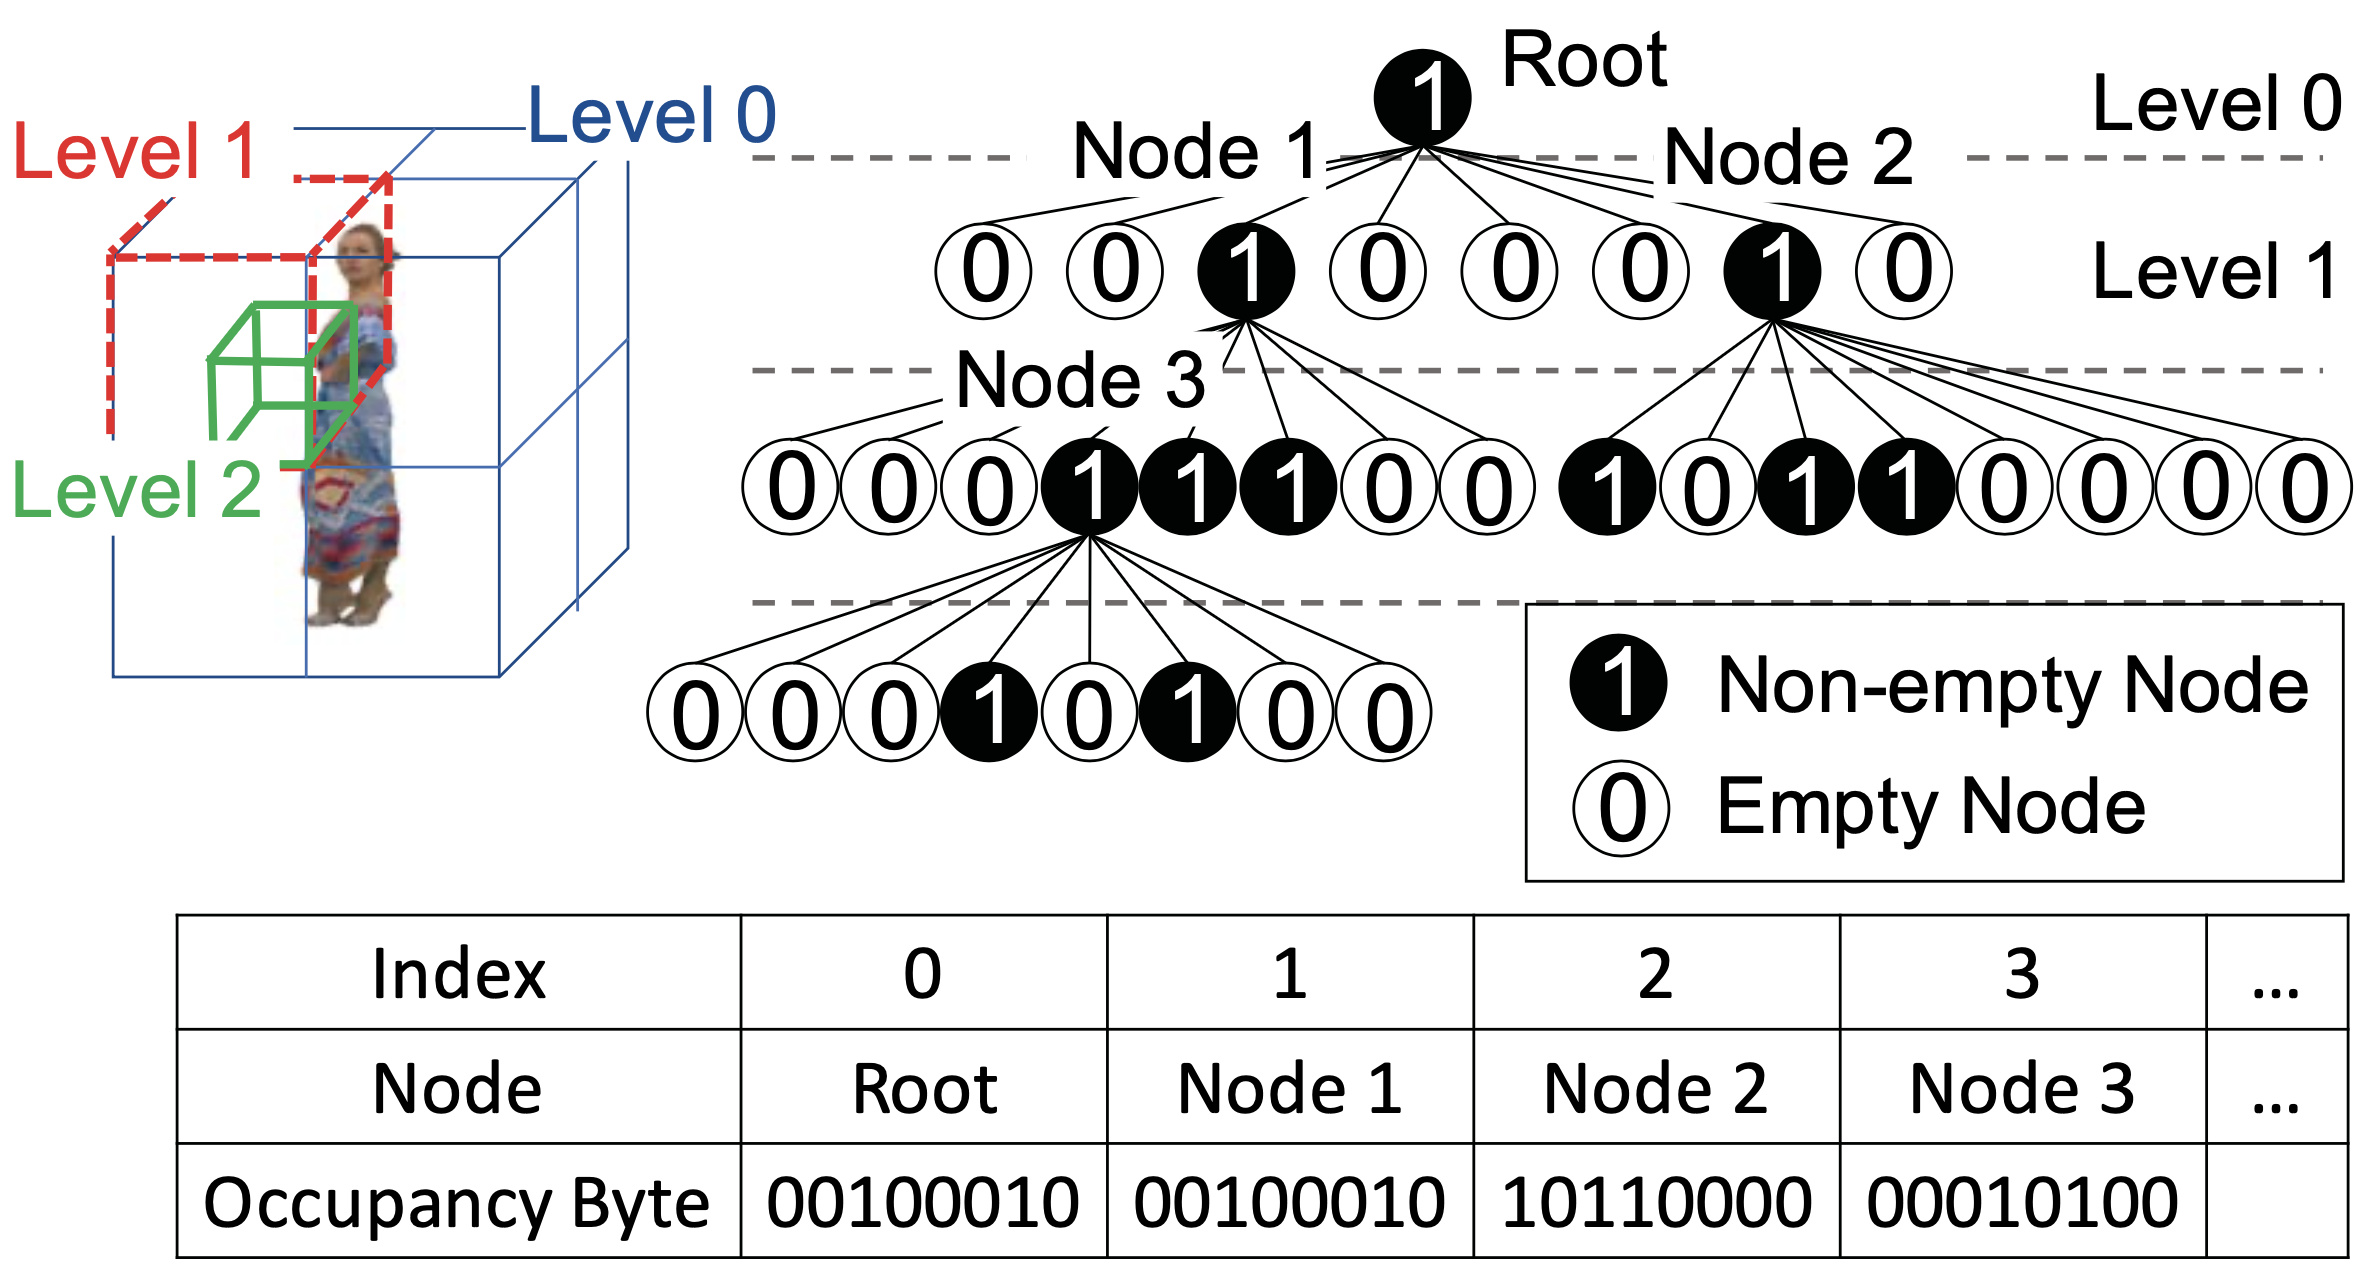
\includegraphics[width=\columnwidth]{figures/octree.png}
  \caption{Octree. \raj{Taken from GROOT paper. Replace it with yours}}
  \label{fig:octree}
\end{figure}
%
Given voxelized 3D space, many voxels are empty and only a small fraction of voxels are occupied by Gaussians.
%
Octree coding is a widely used data structure that efficiently encode the positions of occupied voxels to exploit sparsity and spatial locality.
%
It recursively partitions the 3D space into octants (8 equally-sized child nodes), creating a tree structure where each node represents a cubic region of space that is occupied. Consider the octree in \cref{fig:octree}.
%
The root node represents the entire 3D space, and its 8 child nodes represent the 8 equally-sized children.
%
If the root node is represented as a byte, then each bit indicates whether the corresponding child node is occupied (1) or empty (0). For example, if the third and seventh bits are set to 1, it means that the third and seventh child nodes are occupied, while the rest are empty.
%
The child nodes that are occupied can be further subdivided into their own child nodes, and the process continues recursively until we reach a leaf node that contains a single occupied voxel or an empty node. 

Given our voxelized \gs model, we can coonstruct such an octree by starting from the root node that represents the tight bounding box with dimension $2^J \times 2^J \times 2^J$.
%
The leaf nodes of the octree correspond to the occupied voxels in the voxelized \gs model.
%
Thus, $J$ is the depth of the octree, and the number of leaf nodes is equal to the number of occupied voxels $\hat{N}_v$.

Every node of an octree can be represented as a occupany byte, where each bit indicates whether the corresponding child node is occupied or empty.
%
The octree can be encoded into a bitstream by traversing the tree in level-order and writing the occupancy bytes of all nodes at each level contiguously.
%
Since, occupany bytes only encode nodes that are occupied, the total number of bytes required to encode the octree is proportional to the number of occupied voxels $\hat{N}_v$, which is much smaller than storing all $2^{3J}$ voxels.
%
This makes octree coding an efficient way to encode the positions of occupied voxels in a compact bitstream. The decoder can reconstruct the octree by reading the occupancy bytes level by level and determining which child nodes are occupied based on the bits set to 1.

\parab{RAHT.}
%
Region-Adaptive Hierarchical Transform (RAHT) is an orthogonal transform designed for sparse, non-uniform point cloud data attributes \cite{de2016compression}.
%
It can be intuitively understood as an extension of the  Haar wavelet transform to a sparse 3D grid.
%
%
RAHT adapts to this sparsity by using the underlying Octree structure of the geometry, resulting in a unique RAHT transform for each voxelized geometry.  

The core principle of RAHT is to represent attributes as a signal over the occupied voxels.
%
As illustrated in \cref{fig:raht}, the algorithm processes pairs of sibling nodes that share a common parent in the Octree.
%
For any two sibling nodes $i$ and $j$ with attribute values $a_i, a_j$, RAHT decomposes the signal into: 
\begin{enumerate}
    \item \textbf{Low-frequency Coefficient:} A weighted average representing coarse signal information. 
    \item \textbf{High-frequency Coefficient:} A weighted difference representing the signal details
\end{enumerate}

The process above is repeated for each pair of sibling nodes at a given octree level. 
The low-frequency coefficients are propagated to their parent in the octree, while the high-frequency coefficients are quantized. This process is repeated for each level of the octree.
For smoothly varying spatial signals (e.g., colors in point clouds), this process results in high-frequency coefficients near zero, that can be effectively quantized and entropy codec. 

%

RAHT can be applied to any attributes of a point cloud, typically it is applied to color. 
%
We show that RAHT can also be effective for compressing \gs attributes including opacity, scale, rotation, and color (represented as spherical harmonics).
%
% RAHT is even more effective for \gs since it allows high compressibility for all these attributes using entropy coding.

\parab{RAHT prelude.}
\eduardo{I would move this to the other section. The prelude was not in the original RAHT paper from  (de Queiroz and chou), that I added earlier.  When you introduce the parallel RAHT, you can mention the prelude and say that we need this new approach to effectively parallelize RAHT.}
%
In the original RAHT formulation, the transform is strictly dependent on the siblings of each node in the octree.
%
A parent node in the octree might have anywhere from one to eight occupied children.
%
The prelude step must scan the grid and identify which nodes are siblings.
%
If a node is the only child, it has no sibling, and its value is promoted without transformation.
%
If multiple siblings exist, they must be paired.
%
The RAHT prelude is pre-processing step that helps finding sibling pairs with corresponding weights for the RAHT transform.

\parab{Entropy coding.}
%
After RAHT, the attribute coefficients are quantized and then entropy coded to generate the final bitstream.
%
Quantization of an attribute $a$ is given by the following:
% 
\[\hat{a} = \mathrm{sign}(a) \cdot \left\lfloor \frac{|a| + qp_a/4}{qp_a} \right\rfloor\]
%
where $qp_a$ is called the \textit{quantization step} for attribute $a$.
%
A smaller $qp_a$ results in finer quantization and higher visual quality, but also larger bitstream size and vice versa.

Inspired by G-PCC~\cite{gpcc}  we use Run-Length Golomb-Rice (RLGR) entropy coding.
%
\eduardo{make sure you include the GPCC acronym earlier}
%
RLGR combines run-length encoding, which compresses consecutive repeated symbols, with Golomb-Rice coding, which is effective for encoding integers with a geometric distribution.
%
This makes RLGR particularly suitable for encoding the quantized coefficients from RAHT, which often contain long runs of zeros (high-frequency coefficients) and a few non-zero values (low-frequency coefficients).
%
By applying RLGR, we can further reduce the size of the compressed bitstream while preserving all the information needed for lossless reconstruction of the attributes.
%
Though RLGR is lossless, the quantization step before RLGR is lossy, and the level of quantization can be adjusted to achieve different trade-offs between compression ratio and visual quality.

\subsection{Parallelized Octree Encoding}\label{sec:octree-encode-gpu}
Traditionally, octree is used to hold $(x,y,z)$ positions of points in a point cloud. 
%
Octree based encoding consists of 2 steps: (a) octree construction and (b) bitstream generation.
%
Octree construction starts with voxelized positions (within tight bounding box around the point cloud) and builds a tree structure by recursively subdividing the 3D space into octants~\cite{octree-orig1982,gpcc}.
%
Due to sparse distribution of points, octree data structure efficiently holds only the occupied voxels, which is much smaller than all the voxels in the 3D space.
%
The depth of the octree $J$ is determined by the resolution of the voxel grid, and the leaf nodes correspond to the occupied voxels, which holds the voxelized positions.
%
The octree is then encoded into a bitstream to generate the final compressed representation of the geometry.
%
Each node of the octree represented by an occupancy byte, where each bit indicates if a child node (out of 8 children) is occupied, given by 1, or empty (given by 0).
%
A child is occupied if there is at least one point in its octant.
%
The occupancy bitstream is generated by traversing the octree in level-order and writing the occupancy bytes of all nodes at each level contiguously~\cite{octree-comp2002,octree-comp2006}.
%
The occupancy bitstream is further compressed using entropy coding techniques such as RLGR to generate the final compressed geometry bitstream~\cite{gpcc}.

Decoding the compressed bitstream to extract the voxelized positions first involves entropy decoding followed by reconstructing the octree structure from the occupancy bytes.
%
To help the decoder reconstruct the octree, the encoder needs to add metadata to the bitstream header such as the depth of the octree $J$, and the number of nodes at each level of the octree.
%
The decoder starts from the root node and reads the occupancy bytes level by level to determine which child nodes are occupied based on the bits set to 1.
%
At each level, the decoder finds the number of occupied nodes using the metadata and extracts the occupancy bytes for each node (parent). 
%
For each of these parent nodes, it adds a child to the octree for each bit set to 1 in the occupancy byte, and adds the child node to the list of nodes to be processed at the next level.
%
This process continues until the decoder reaches the leaf nodes at depth $J$, which correspond to the occupied voxels.
%
The reconstructed voxelized positions are then obtained by calculating the center coordinates of the leaf node voxels.

%
Today, 2D video codecs such as H.264 and H.265 are implemented on GPU, which allows for real-time encoding and decoding of high-resolution videos.
%
Since \gs data inherently resides in GPU memory during training and rendering, it is critical to implement the entire compression pipeline on GPU to avoid costly memory copy between CPU and GPU.
%
The first step in to develop a highly parallel octree encoding algorithm that can be efficiently implemented on GPU.

\parab{Challenges.}
%
Octree construction building from root to leaf using the traditional recursive approach is inherently sequential.
%
State of the art octree encoding algorithms in ~\cite{gpcc,draco,pcl} are implemented in CPU by building octree in top-down manner.
%
Volumetric video streaming wokrs such as ViVo~\cite{vivo}, MeshReduce~\cite{meshreduce}, and MetaStream~\cite{metastream} exploit CPU parallelism by partitioning the 3D space into exclusive blocks and building octree independently for each block.
%
The parallelization challenges in octree encoding occurs in 3 stages: octree construction, bitstream generation, and decoding bitstream.
%
Building the octree requires traversing the tree top-down and creating nodes and pointers, which is difficult to parallelize on GPU due to irregular memory allocation and pointer chasing with poor locality~\cite{octree-gpu2011,octree-cpu2020,groot}.
%
Again, generating the occupancy bitstream requires tree traversal in level-order and pointer chasing to determine the occupancy byte of a node depending on existing children.
%
Similarly, the decoder requires requires traversing the bitstream and recursively building the tree top-down~\cite{octree-cpu2020,groot}.
%
We present arguments from prior work on octree parallelization in \cref{tab:octree-challenge}.

Prior works~\cite{octree-cpu2008,octree-gpu2011,octree-gpu2012} have attempted to parallelize the octree construction by constructing the tree from leaf to root.
%
The key idea is to linearlize the positions in 3D to a 1D list using morton codes, which is a space-filling curve that maps 3D coordinates to a single dimension while preserving spatial locality~\cite{morton-code-spc}.
%
morton codes allow for $O(1)$ parent-child determination, which enables parallel construction of the octree without explicit nodes and pointers.
%
The generated octree is not explicitly represented as a tree structure, but rather as arrays of morton indices for each node at a certain level. 
%
These works used this representation for fast neighbor selection~\cite{octree-gpu2012} and surface reconstruction~\cite{octree-gpu2011}, but they did not generate the occupancy bitstream which is required for octree-based compression.
%
This still need to be generate in CPU~\cite{gpcc,draco}.
%
Recent works~\cite{octree-cpu2020,groot} have attempted only to parallelize the entire octree encoding using CPU or hybrid CPU-GPU, but they can only paralleize a very few levels near the leaf level, and the rest of the levels are still generated sequentially on CPU.

\begin{table}[h]
  \centering
  \begin{tabular}{lp{0.7\columnwidth}}
    \hline
    \textbf{Works} & \textbf{Quote}  \\ \hline
    Zhou~\cite{octree-gpu2011} & ``Creating an octree for point clouds directly on the GPU, however, is very difficult, mainly because of memory allocation and pointer creation.'' \\ \hline
    GROOT~\cite{groot} & ``While the tree structure efficiently handles the sparsity of 3D data and subdivides only the volumes where the point exists, the irregularity requires traversing the serialized byte stream and recursively calculating the child node geometry. The exact positions that represent intermediate nodes depend on the occupancy of their ancestors, which cannot be parallelized.'' \\ \hline
  \end{tabular}
  \caption{Parallelization challenges for octree encoding reported in prior work}
  \label{tab:octree-challenge}
\end{table}

\parab{Morton codes.}
\begin{figure}[t]
  \centering
  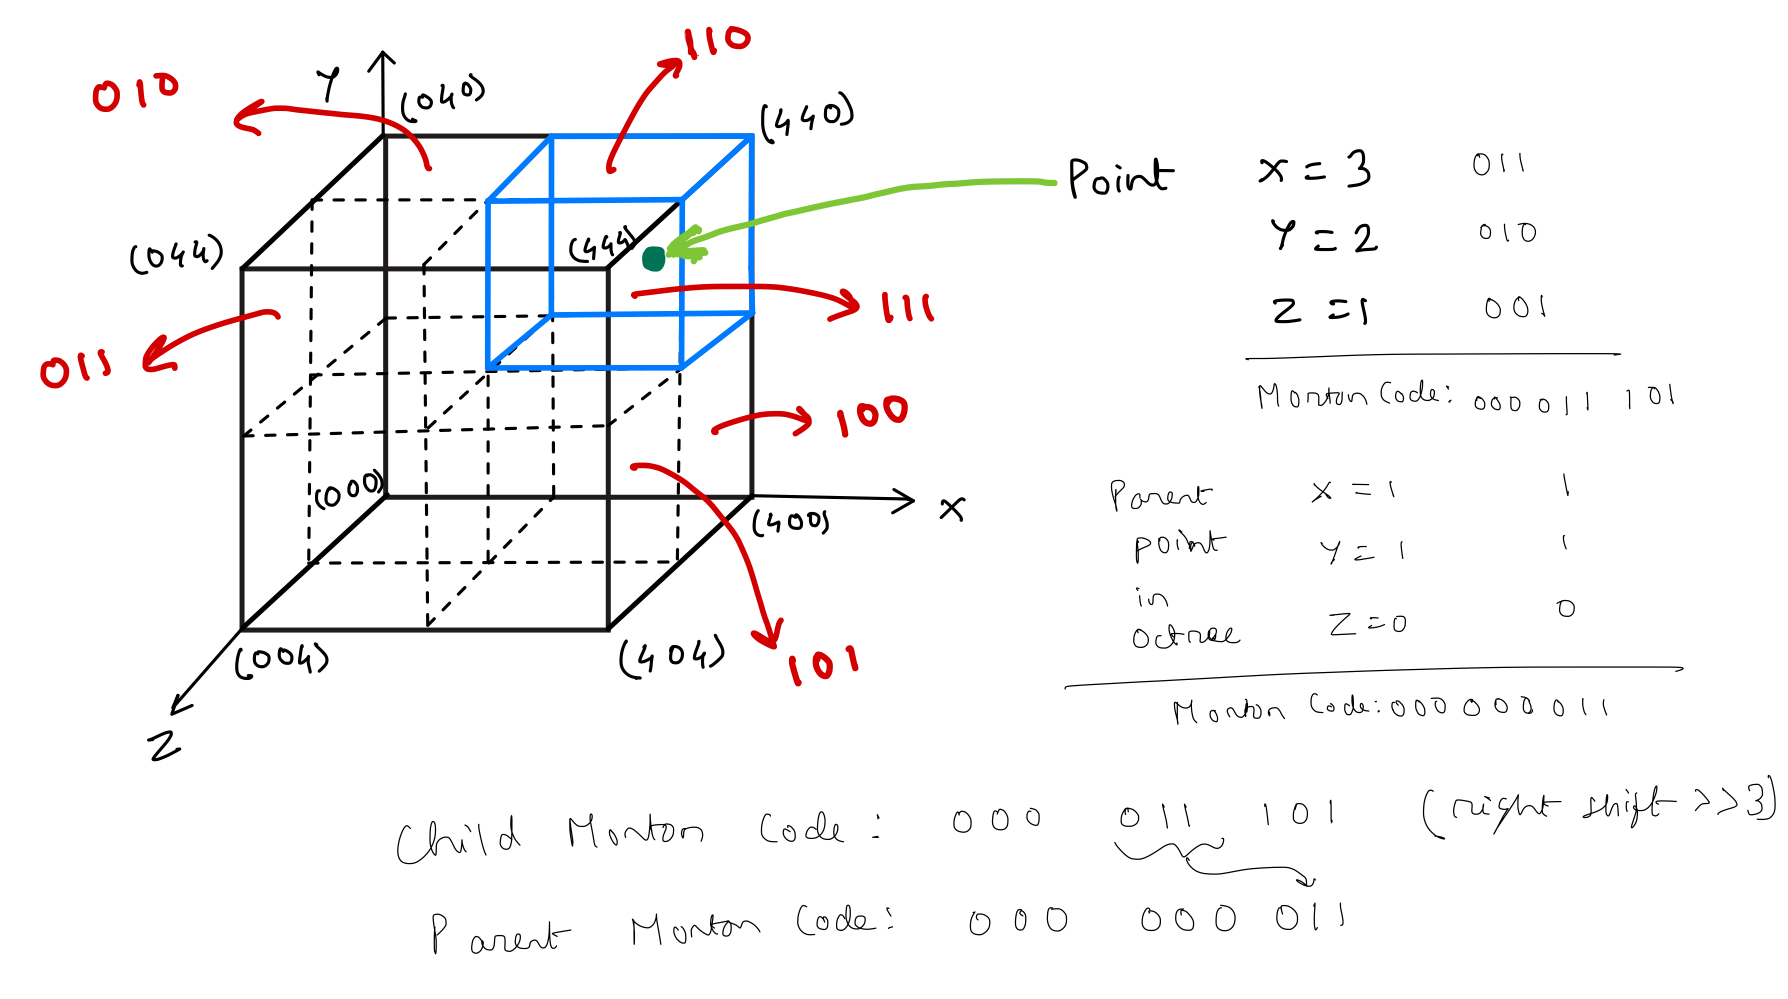
\includegraphics[width=\columnwidth]{figures/morton.jpeg}
  \caption{Undestanding morton codes. \raj{Replace it with your drawio figure}}
\label{fig:morton}
\end{figure}
%
Following prior works~\cite{octree-cpu2008,octree-gpu2011,octree-gpu2012}, the key to our GPU design is to never build explicit tree pointers.
%
Instead, we represent each occupied voxel by its \emph{morton code}, which is the bit-interleaving of its integer voxel coordinates.
%
For a voxelized coordinate $\hat{v}=(x,y,z)\in\{0,\ldots,2^J-1\}^3$, the morton code is a bit string $x_{J-1}y_{J-1}z_{J-1}\ldots x_0y_0z_0$ where $x_b,y_b,z_b$ are the $b$-th least-significant bits of $x,y,z$.

Morton codes has two properties: (a) linearize 3D occupancy while preserving spatial locality: voxels that are close in space tend to be close in the sorted morton order~\cite{morton-code-spc}, (b) make octree topology \emph{implicit}: if $c_m$ is morton code for child node, its parent's code $p_m$ is simply $p_m = c_m \gg 3$, \ie dropping the last three interleaved bits; conversely, if $p_m$ is a parent code, its eight candidate children have morton codes $[(p_m \ll 3) \;|\; i]_{i=0}^7$, where $i$ is the child index.
%
Consider the example in \cref{fig:morton}, where we have a $4\times4\times4$ voxel grid ($J=2$) with one occupied voxel.
%
Let's consider the morton code for the root node, which the bounding box of the entire grid, is 0. 
%
The bounding box gets subdivided into 8 child octants, thus the child morton codes $[000,001,\ldots,111]$ uniquely identify each child.
%
If one of the child octants is occupied, say the one with morton code 5, then its parent code is simply $5 \gg 3 = 0$ (root node), which is the root node.
%
If the octant with morton code 5 is further subdivided, its children have morton codes $[40,41,\ldots,47]$, which can be computed by left-shifting the parent code and adding the child index, \ie $5 \ll 3 = 40$ is the first child, and $5 \ll 3 + 7 = 47$ is the last child.
%
Conversely, the parent code of any of these children is simply $[40,41,\ldots,47] \gg 3 = 5$.
%
If we carefully observe, morton codes for the occupied voxel act as indices to the octree nodes as octants are subdivided.
%
Thus, morton codes provide an $O(1)$ arithmetic mapping between a node and its parent/child codes.
%
This is the critical property that removes pointer chasing and makes the octree GPU-friendly.

\parab{Octree construction.}
%
The input to octree encoding is the voxelized \gs positions~\ref{sec:background}, \ie integer voxel centers $\hat{V}=[\hat{v}_i]_{i=1}^{\hat{N}_v}$ already stored in GPU memory as a tensor $[\hat{x}_i,\hat{y}_i,\hat{z}_i]$.
%
The first step is to compute the morton code for each integer position.
%
We launch one CUDA thread per integer voxel to compute its morton code by bit interleaving $x_{J-1}y_{J-1}z_{J-1}\ldots x_0y_0z_0$, where $J$ is the octree depth.
%
We use a 64-bit morton code to support octree depths up to $J=21$, which is sufficient for a decent scene size~\cite{mesongs}.
%
If $J\leq 21$, the unused most-significant bits in the morton code are simply set to 0.

The list of morton codes for the integer voxels become the leaf nodes of the octree.
%
We sort the list of morton codes in parallel using CUDA radix sort.
%
Sorting brings all the neighboring voxels together.
%
Now, the octree construction starts from sorted list of morton codes, $L_J$.

At depth $J-1$, the parents of the leaf nodes need to be identified.
%
Recall that shifting a morton code right by 3 bits gives the parent code.
%
Each thread can independently compute the parent code $p_m$ from the morton code of a leaf node $c_m$ by right-shifting its morton code by 3 bits, $p_m = c_m \gg 3$.
%
Since the morton code is sorted and bit right-shift preserves the order, the parent morton codes are also sorted but not unique.
%
Unlike other GPU octree construction tecnhniques~\cite{octree-cpu2008,octree-gpu2011,octree-gpu2012}, we only sort the leaf nodes, and we never sort the internal nodes.
%
But, multiple leaf nodes can have the same parent code, so we need to compact duplicates to get the unique parent codes.
%
We use CUDA's unique primitive to compact duplicates in parallel, which gives us the list of occupied parent nodes at depth $J-1$.
%
Similar to leaf level, we arrive at a list of unique sorted morton codes for the occupied nodes at depth $J-1$.
%
We repeat this process iteratively until we reach the root node at depth 0, which has a single code 0 for the root node.

\parab{Bitstream generation.}
%
Like past works~\cite{octree-cpu2008,octree-gpu2011,octree-gpu2012}, we do not build an explicit tree structure with pointers on GPU.
%
This means each node doesn't have an explicit occupancy byte that can be directly written to the bitstream.

The output of octree construction is a list of morton codes for the occupied nodes at each level, \ie $L_0,\ldots,L_J$, where $L_0$ has the root node, $L_J$ has the leaf nodes, and $L_d$ has the occupied nodes at depth $d$.
%
From these lists, the encoder must emit the octree occupancy bitstream.
%
Each internal node contributes exactly one occupancy byte, whose $i$-th bit is set if child $i$ exists.
%
Given a parent code $p_m\in L_d$, the base code of its children can be obtained by $c_m = p_m \ll 3$ exploiting the property of morton code.
%
The eight possible children are therefore the contiguous code range $[c_m,c_m+7]$.
%
To compute the occupancy byte for $p_m$, we need to check which of these eight candidate child codes exist in the child list $L_{d+1}$.
%
This requires searching for the child codes in $L_{d+1}$.
%
We make 2 observations that make this search efficient. 
%
First, all actual children with morton codes in the range $[c_m,c_m+7]$ must appear contiguously in the sorted list $L_{d+1}$.
%
Second, we can perform a binary search to find the first occupied child code $\geq c_m$ in $L_{d+1}$.

The octree encoder launches a CUDA kernel with one thread per parent node in $L_d$.
%
It starts with a occupancy byte initialized to 0.
%
Each thread performs the following steps:.
(i) compute $c_m = p_m \ll 3$;
(ii) binary-search $L_{d+1}$ to find the first occupied child code $\geq c_m$;
(iii) scan forward over at most 8 entries until the child code exceeds $c_m+7$;
(iv) set bit for every child code $c_m$ found.
%
Thus, each thread writes exactly one occupancy byte.
%
Once the kernel completes, the occupancy bytes for all nodes at level $d$ are stored in a GPU buffer.
%
The above steps are repeated from the root level down to the leaf level, \ie in level order, where each level is processed in parallel.
%
We present the detailed algorithm in \cref{algo:octree-encode-gpu}.

\parab{Parallelization template.}
Our parallelization strategy for octree construction is a simple level-synchronous approach. 
%
At each level, we launch one thread per node to perform a computation, then we gather the results in a list. 
%
This list is used to launch the next level of threads, and we repeat this until we reach the root node. 
%
We will use such level-synchronous heirarchy template for most of \gsnfs's algorithms, including RAHT, which we will describe later.

\subsection{Parallelized Octree Decoding}\label{sec:octree-decode-gpu}
Given the encoded bitstream obtained from the above octree encoding process, the decoder need to extract the voxelized positions.
%
Note that the voxelized positions are not explicitly stored in the bitstream, but rather implicitly represented by the center of the leaf node voxels in the octree.
%
The decoder extracts the occupancy bytes from the bitstream sequentially, starting from the root node and traversing the octree level by level.
%
At each level, the decoder reads the occupancy byte for each parent node to determine which child nodes are occupied.
%
It adds the adds the occupied child node to the octree and continues this process until it reaches the leaf nodes at depth $J$, which correspond to the occupied voxels.
%
The decoder can reconstruct the voxelized positions by calculating the center coordinates of the leaf node voxels.

\parab{Challenges.}
The decoder needs to read the occupancy bytes sequentially and build the octree top-down, which is difficult to parallelize on GPU due to irregular memory allocation and pointer chasing with poor locality.
%
GROOT~\cite{groot} argues that ``the number ofnodes at each octree depth is determined by the number of occupiedbits among the nodes at the parent-depth, which requires sequential decoding''.
%
GROOT and~\cite{octree-cpu2020} tries to achieve some parallel decoding for a few lower levels of the octree, but the majority of the levels are still decoded sequentially on CPU in a top-down manner.
%
A first attempt to parallelize the octree decoding is to follow the same level-synchronous approach as the encoder, where we launch one thread per parent node at each level to determine the occupied child nodes and build the octree bottom-up.
%
However, this approach can only work if the morton codes for the occupied child nodes at each level are explicitly stored in the bitstream.
%
Storing morton codes in the bitstream would require 64-bits per occupied node, which is much larger than the 1 byte per node required by the occupancy bitstream.

\parab{Octree decoding.}
Our key insight is that morton codes can be generated on the fly during decoding without explicitly storing them in the bitstream.
%
The morton code for the root node is always 0 and its children will have have morton codes $[0,1,\ldots,7]$.
%
While decoding the occupancy byte for the root node, we can determine which child nodes are occupied and generate their morton codes by left-shifting the parent code and adding the child index (bit position that is set to 1).
%
This will generate a list of morton codes for the occupied child nodes at the first level.
%
For subsequent levels, we can repeat the same process level-by-level.
%
Thus, once we know which child indices are occupied (from the occupancy byte), we can generate the exact Morton code of every occupied child in $O(1)$ time without any tree pointers.
%
This on-the-fly morton code generation is the core mechanism that makes decoding both GPU-friendly and memory efficient.
%

\gsnfs uses the same level-synchronous approach as the encoder, where we launch one thread per parent node at each level to determine the occupied child nodes and generate their morton codes.
%
But, each parent has a variable number of occupied children, ranging from 0 to 8 depending on sparsity.
%
Therefore, the morton code list for the next level $L_{d+1}$ is a variable-length concatenation of each parent's children.
%
On the GPU, variable output sizes require computing write offsets so that each parent thread writes its children into a disjoint region of the output array without atomics.
%
We compute these offsets via a prefix sum over the per-parent child counts.
%
Each element of the prefix sum provides the indices to the children's list, where the parent thread writes the morton codes of its occupied children.

The decoder extracts the octree depth from the first 4 bytes of the bitstream header and the number of nodes at each level from the next $4J$ bytes of the header.
%
At each level, the decoder reads the occupancy bytes for all nodes at that level from GPU memory.
%
Then, it launches a CUDA kernel that counts the number of occupied children for each parent node by counting the number of set bits (using population count CUDA primitive) in the occupancy byte.
%
From the child counts, we compute the write offsets for each parent node by performing a parallel prefix sum.
%
Again, it launches a CUDA kernel with one thread per node to generate the morton codes for its occupied children.
%
It writes the codes at the offsets calculated by the prefix sum.
%
After processing all levels, the decoder has the list of morton codes for the leaf nodes, which correspond to the occupied voxels.
%
It launches a final CUDA kernel to decode the morton codes back into integer voxel coordinates by reversing the bit interleaving.

\raj{Add complexity analysis of octree encoding and decoding.}
\raj{Ramesh: While going through this section, can you please suggest places where we can add figures to make the explanation clearer?}
\raj{Ramesh: Do we need to write a paragraph on ANS entropy coding on octree bitstream or should we only put a 1-liner here? Alternatively, we can add it here \cref{sec:entropy-coding}}

\subsection{Parallelized RAHT}\label{sec:raht-encode-gpu}
\begin{figure}[t]
  \centering
    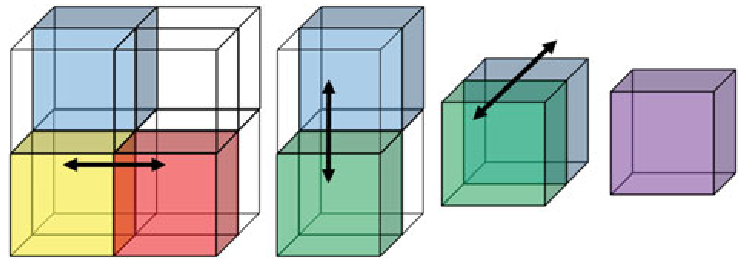
\includegraphics[width=\columnwidth]{figures/raht.png}
    \caption{One level of RAHT applied to eight adjacent voxels (colored are occupied). \raj{Taken from Eduardo's paper. Replace it with yours}}
  \label{fig:raht}
\end{figure}
%
A \gs frame contains a set of Gaussians (one per occupied voxel), each having attributes such as scale, rotation, opacity, and color.
%
For degree 3 SH, there will be $3 + 4 + 1 + 48 = 56$ attributes that.
%
These attributes are spatially correlated: neighboring voxels often have similar opacity and geometry attributes, and smooth surfaces induce slowly varying SH coefficients.
%
Naively entropy coding the raw attributes waste bits because it ignores this correlation, leading to poor compression efficiency.
%
To exploit spatial correlation, \gsnfs applies a transform coder---analogous to DCT/wavelets in 2D video---that concentrates most attribute energy into a small number of low-frequency coefficients and produces many near-zero high-frequency residuals that are highly compressible.
%
G-PCC applies uses  RAHT-based transform coding for voxelized point attributes such as color. 
%
Similarly, for each 3DGS we build the RAHT on top of the voxelized geometry and apply it to the remaining \gs attributes. 
%
RAHT applies a sequence of orthonormal $2\times 2$ transforms to attributes living on the \emph{occupied} leaf voxels, proceeding bottom-up from leaves to the root; the inverse transform runs in the reverse order.\eduardo{this paragraph above describing 2x2 transforms can be moved to the how raht works subsection below.}

\parab{How RAHT works.}
We illustrate the forward RAHT using the canonical example in Fig.~\ref{fig:raht}. 
%
Consider a $2 \times 2 \times2$ cube where only three of the eight voxels are occupied (colored voxels in the figure). 
%
The attribute (say opacity) in three colored voxels has values $a_r,a_y,a_b$ (red, yellow, and blue, respectively) and an initial unit weight of $w_r,w_y,w_b$.
%
At a certain level in the octree, RAHT processes sibling voxel pairs axis-by-axis ($x$, then $y$, then $z$). If a voxel has no neighbor along the current axis, its coefficient is copied forward unchanged \eg the blue voxel in the $x$-axis.
%
Note that attribute values are only located at leaf, so RAHT applies the transform bottom-up from leaf level to root.
%
\raj{Mark the 3D axes in the figure and show the axis-by-axis processing.}
%
If two neighbors exist \eg red and yellow, RAHT applies the orthonormal transform, given by the equation:
\begin{equation}
  \begin{bmatrix}
  a_g^0\\
  a_g^1
  \end{bmatrix}
  =
  \frac{1}{\sqrt{w_y+w_r}}
  \begin{bmatrix}
  \sqrt{w_y} & \sqrt{w_r}\\
  -\sqrt{w_r} & \sqrt{w_y}
  \end{bmatrix}
  \begin{bmatrix}
  a_y\\
  a_r
  \end{bmatrix},
  \label{eq:raht-butterfly}
\end{equation}
where $a_g^0$ is the low-frequency (coarse) coefficient and $a_g^1$ is the high-frequency (detail) coefficient.
%
After the transform, both coefficients will have updated weights $w_g = w_y + w_r$ (green cube). 
%
The coefficient $a_g^1$ is stored for entropy coding along with its weight, while $a_g^0$ is further processed and put in the green cube.
%
For processing along the $y$-axis, the green and blue voxels do not have neighbors, so their values are copied to the next level.
%
RAHT applies the same transform~\ref{eq:raht-butterfly} to the green and blue voxels along the $z$-axis with weights $w_g$ and $w_b$.
%
It repeats this process for each voxel in $2 \times 2 \times2$ cube at each level of the octree. 
%
After $J$ levels, the low-frequency coefficient moves to the root and remaining nodes contain high-frequency coefficients.
\eduardo{RAHT coding pipeline figure: It may help implementation explanations to not input attributes to RAHT prelude, but to input it directly to RAHT transform. You can do that by making two arrows out of voxelization+merging, one outputing positions and the other outputing all attributes. }
\begin{figure}[t]
  \centering
    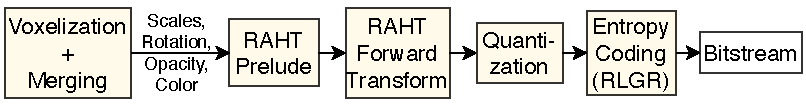
\includegraphics[width=\columnwidth]{figures/raht_pipeline.pdf}
    \caption{RAHT coding pipeline.\eduardo{This figure should have the KLT.}}
  \label{fig:raht-pipeline}
\end{figure}
%
Because weights are accumulated whenever two coefficients (in sibling pairs) merge, the low-frequency coefficient ends with the largest weight, while high-frequency coefficients produced early have smaller weights.
%
These weights depend only on the octree structure (not on the attribute values), and thus provide a natural frequency ordering for the coefficients.
%
Last step is sorting the RAHT coefficients by decreasing weight before quantization and entropy coding; full pipeline in~\cref{fig:raht-pipeline}.
%
\eduardo{this is not what we do, the ordering is different, I think you explained it earlier in the paper.}

\parab{RAHT prelude.}
%
A naive RAHT implementation would explicitly traverse the octree and discover sibling pairs at each transform step \cite{de2016compression,gpcc}.
%
This is inefficient since it requires sequential tree traversal.
\eduardo{I think this is also inefficient because you do this for ever attribute.  Prelude allows you to figure out all these indices only once, and then you reuse them to apply the RAHT to all attributes. }
%
Instead, the implementation from~\cite{raht} computes a \emph{prelude} step before running the RAHT transform. 
%
This finds the indices to per-layer pairs from the morton-ordered voxels.
%
Concretely, given a voxelized 3D space with morton codes for each voxel, the prelude computes, for each layer $\ell \in \{1,\dots,3J\}$ (3 denotes the number of axes):
%
(i) an index list $I_\ell$ indicating the active coefficients at that layer,
%
(ii) a weight list $W_\ell$ for those active coefficients, and
%
(iii) a flag list $F_\ell$ indicating which active coefficients are left siblings (\ie should be paired with the next coefficient).
%
Once the prelude $(I_\ell,W_\ell,F_\ell)$ is available, the forward RAHT is just a sequence of independent $2\times2$ matrix-vector products applied to the sibling pairs at each level.

\parab{RAHT algorithms.}
Before we describe the parallelization, we first explain the RAHT prelude and transform at a high level. The explicit algorithms are presented here~\cref{algo:raht-prelude,algo:raht-forward}.

RAHT operates on pairs of sibling voxels, more precisely on the sibling coefficients.
%
Therefore, at each transform step, RAHT must know which coefficients should be paired and what weights they carry.
%
A naive implementation would traverse the octree and discover siblings on the fly, but this is sequential and pointer-heavy.
%
Instead, the RAHT prelude converts the Morton codes for the voxels as indices to the octree.
%
To recall, the bits of the Morton code for a octree node indicate the path from the root to that node, and also two nodes are siblings if their prefixes match up to a certain bit, given by level $\ell$.
%
At each step $\ell$, where $1 \le \ell \le 3J$ (3 is due to 3-axes), RAHT prelude computes three lists:
%
(a) a list of currently active coefficient indices ($I_\ell$),
%
(b) a boolean indicator that marks which active coefficients are left siblings ($F_\ell$), and
%
(c) an integer weight per active coefficient ($W_\ell$) that tracks how many leaf voxels are represented by that coefficient.
%
Intuitively, $I_\ell$ says which coefficients exist at this step, $F_\ell$ says which adjacent coefficients should be paired, and $W_\ell$ provides the pair weights used in Eq.~\ref{eq:raht-butterfly}.
%
The prelude (Alg.~\ref{algo:raht-prelude}) essentially computes these by scanning adjacent Morton codes: if two adjacent Morton codes share the same prefix at the current step, the earlier one is flagged as a left sibling, and the later one becomes its right sibling; right siblings are then removed to form the next active list.

The forward RAHT is a sequence of independent $2\times2$ weighted orthonormal transforms (weights obtained from the prelude) applied to sibling pairs at each step (Alg.~\ref{algo:raht-forward}).
%
For each left sibling in $F_\ell$, RAHT identifies if its sibling pair exists in the next active coefficient in $I_\ell$, and applies the weighted transform in Eq.~\ref{eq:raht-butterfly} across all attribute dimensions.
%
This produces one coefficient that is propagated upward (low-frequency) and one coefficient that is kept (high-frequency).
%
Inverse RAHT transform runs the same steps in reverse order and applies the inverse of Eq.~\ref{eq:raht-butterfly} (the transpose of the forward matrix), reconstructing the attributes.

\parab{Why RAHT needs to be parallelized.}
A \gs frame has many attribute dimensions: opacity is a scalar, rotation has 4 quaternions, scale has 3 axes, and color has 48 SH coefficients (up to degree 3).
%
This means that RAHT needs to be applied to each attribute dimension.
\eduardo{below I think you should mention across which dimensions you want/can exploit parallelization in raht and prelude, and then say the challenges and how you solve it. I think the parallelizable directions are 1) acrsoss attributes, 2) within each octree level. Across octree levels is sequential, and that introduces the difficulty you describe in more detail below.}
\parab{How \gsnfs parallelizes the prelude.}
The prelude’s main challenges are (a) sparsity causing irregular sibling structure and (b) the active list shrinking unpredictably across steps.
%
\gsnfs addresses both with similar \emph{level-synchronous} template for octree parallelization~\cref{sec:octree-encode-gpu}. 
%
We describe this below:

\begin{itemize}
\item \textbf{Per-step kernel over a flat list (addresses sparsity).}
%
At each step $\ell$, \gsnfs maintains the current active list $I_\ell$ as a flat GPU tensor of indices.
%
We launch one GPU thread per element of $I_\ell$ to compute $W_\ell$ and $F_\ell$.
%
Each thread compares the Morton code of its current element with the next element (adjacent in Morton order) under the step-specific mask and decides whether they form a sibling pair.
%
Use of Morton codesdoes not require any octree traversal or pointer chasing for sibling discovery, even though occupancy is sparse.

\item \textbf{GPU compaction to form the next list (addresses dynamic list sizes).}
After $F_\ell$ is computed, the next active list $I_{\ell+1}$ is obtained by removing right siblings.
%
\gsnfs implements this efficiently using boolean shift and masked select of tensors which are available in PyTorch (Alg.~\ref{algo:raht-prelude-gpu}).
%
Note that sometimes we use PyTorch primitives and sometimes we write custom CUDA kernels; the choice is based on efficiency and ease of implementation.
%
This matches the level-synchronous template: compute on per-element, then compact the list and relaunch.
\end{itemize}

\parab{How \gsnfs parallelizes the RAHT forward/inverse transform.}
At each step $\ell$ going from $1$ to $3J-1$ (bottom up), RAHT must gather the two coefficient rows of each sibling pair, apply a $2\times2$ transform across all attribute dimension, and write results back in-place; steps are sequential, but work \emph{within} a step is parallel.
%
\gsnfs again follows the level-synchronous template.
%
At step $\ell$, we launch a GPU kernel with one thread per entry in the active list $I_\ell$.
%
Only threads whose flag $F_\ell$ is valid execute the $2\times2$ transform; each such thread reads indices of a sibling pair (current and next element in $I_\ell$), looks up their weights in $W_\ell$, computes the two scalar mixing coefficients, and then applies Eq.~\ref{eq:raht-butterfly} to all attribute dimensions.

Inverse RAHT uses the same schedule $(I_\ell,F_\ell,W_\ell)$ and the same per-step parallel kernel structure.
%
The only differences are (i) the order of steps (top-down, i.e., reverse $\ell$) and (ii) using the inverse $2\times2$ transform.
%
Therefore, the inverse inherits the same parallelization benefits and does not introduce additional structural complexity.

\subsection{Quantization}\label{sec:quantization}
Video codecs rely on quantization to trade visual quality for compression gains by mapping continuous-valued signals to a smaller set of discrete levels.
%
Entropy coders map these discrete values to a binary bitstream. Coarser  quantization leads to a  smaller  set of discrete values which reduces the bitstream size.
%
For \gs, this is particularly important because each Gaussian carries a high-dimensional attribute (opacity, rotation, scale, and SH), and many of them vary smoothly over space---meaning that small difference in attribute value often have limited perceptual impact once rendered.
%
In \gsnfs, we apply quantization on the attributes after RAHT because RAHT concentrates most attribute energy into a small set of low-frequency coefficients and produces many small-magnitude high-frequency coefficients.
%
It pushes the high-frequency coefficients to zero, creating long zero runs that entropy coders like RLGR compresses efficiently.
%
We do not quantize positions because geometry is already compactly represented by the octree bitstream (which is lossless in \gsnfs) and because small position perturbations can introduce artifacts in scene geometry (e.g., popping/flicker) that are more noticeable than errors in appearance.
\eduardo{this above does not make sense. The RAHT cannot be used to compress positions, because the raht is built on top of the positions. In the system description it should be made very clear that the codec first compresses position, and then compressed all attributes using the positions. This is sometimes called conditional coding, you code attributes conditioned ont he positions, in other words, you assume the positin information is available both at encoder and decoder.}

\parab{How \gsnfs quantizes RAHT coefficients.}
After RAHT, \gsnfs quantizes the RAHT coefficient matrix $C\in\mathbb{R}^{N_v\times D}$, where $D$ is the total attribute dimension, using a dead-zone quantizer that maps to $\hat{C}\in\mathbb{Z}^{N_v\times D}$.
%
Since different attributes have different numeric ranges and perceptual importance, a single quantization step-size would be suboptimal.
%
We use separate quanization step sizes $\Delta_i$, one per attribute group (5 in total)---scale, rotation, opacity, DC SH, and AC SH.
%
We then apply a dead-zone control offset $\delta$ (we use $\delta = 1/4$) and quantize as:
\[
\hat{C_i} = \mathrm{sign}(C_i)\cdot \left\lfloor \frac{|C_i|}{\Delta_i} + \delta \right\rfloor.
\]
%
\eduardo{$\delta$ should be available at encoder and decoer, so it is not transmitted. $\Delta_i$ is also available at decoder and encoder through a table, so what you should actually send is the index. Instead of meta-data use the term overhead. Meta-data is descriptive information about the dataset, while overhead refers to information needed by the decoder to reconstruct the data.}
Given the decoded integers $\hat{C_i}$ and $(\Delta_i,\delta)$ (passed as overhead), the dequantizer applies the transformation:
\[
C'_i = \hat{C_i}\cdot \Delta_i + \mathrm{sign}(\hat{C_i})\cdot\left(\frac{\Delta_i}{2}-\delta\right).
\]

Intuitively, the dead-zone widens the region around zero so that small-magnitude coefficients are more likely to quantize to zero, improving compression with limited visual impact.
%
Finally, before entropy coding, we reorder the quantized coefficients using the RAHT-derived ordering~\cite{raht}, which places low-frequency coefficients before finer high-frequency ones.
%
\eduardo{when you talk about the ordering before you should use this description. We do not do the ordering according to weights If i remember correctly.}
This ordering improves entropy coding efficiency because long runs of zeros are more common among high-frequency coefficients.
%
We implement the dead-zone quantizer using PyTorch primitives to run on GPU.

\subsection{Entropy Coding}\label{sec:entropy-coding}
Entropy coding is the final lossless stage in most codecs: it converts a sequence of quantized symbols into a compact bitstream by assigning shorter codes to more probable symbols and longer codes to less probable ones.
%
We use Run-Length Golomb-Rice (RLGR)~\cite{rlgr} as our entropy coder, which takes the quantized RAHT coefficients $\hat{C}\in\mathbb{Z}^{N_v\times D}$ (after reordering) and outputs a compressed bitstream.
%
RLGR is well suited for quantized RAHT coefficients because it efficiently compresses sequences with many zeros and a small number of non-zero values~\cite{raht,gpcc}.
%
RLGR combines two ideas:
(i) run-length coding for consecutive zeros, and
(ii) Golomb-Rice coding for non-zero magnitudes using an adaptive parameter.
%
\gsnfs uses signed RLGR since RAHT coefficients can be negative.

\parab{GPU-parallel RLGR: block-based parallelism.}
Since all previous stages of \gsnfs runs on GPU, it is critical to implement RLGR encoding and decoding on GPU as well to avoid costly CPU-GPU data transfers.
%
But, RLGR is inherently sequential \emph{within a stream} due to its adaptive state.
%
\gsnfs addresses this by encoding in blocks and running independent RLGR for each block in parallel.
%
We treat the coefficient matrix as $D$ independent channels, each of length $N_v$ symbols, and partition each channel into fixed-size blocks of $B$ (block size) symbols.
%
Each (channel, block) pair is encoded in parallel.
%
Such block-based parallelism achieve lower compression gain than encoding the entire channel, but we found this overhead to be small enough to tradeoff for improved runtime.

\subsection{Decoding}\label{sec:decoding}
Decoding runs the reverse of encoding entirely on GPU in the following order:
(1) RLGR decoding reconstructs the reordered integer coefficient matrix $\hat{C}$;
(2) dequantization maps $\hat{C}$ back to floating-point coefficients;
(3) octree decoding reconstructs voxel positions and morton codes;
(4) RAHT prelude is recomputed from the decoded voxel positions (via morton codes);
(5) inverse RAHT reconstructs the merged per-voxel attributes; and
(6) inverse color-space transform and inverse KLT (\cref{sec:bandw-adapt}) reconstructs SH coefficients, and we reassemble the final \gs parameters.
\eduardo{overhead instead of meta-data?}
\parab{Metadata for decoding.}
To decode a frame, the encoder includes (or the system preserves) the following metadata per frame:
\begin{itemize}
%
\item \textbf{Geometry:} octree depth $J$ and number of occupied nodes per octree level for octree decoding.
%
\item \textbf{Quantization:} per-channel quantization step sizes $[\Delta_i]_{i=1}^5$ and dead-zone offsets $\delta$.
%
\item \textbf{RLGR:} number of channels, symbols per channel, block size, and block offsets to locate each compressed block.
%
\item \textbf{Voxel-to-world mapping:} voxel size and bounding-box dimensions to convert integer voxel coordinates back into world coordinates.
\end{itemize}
